\documentclass[a4paper,12pt, italian]{article}
\usepackage{geometry}
\geometry{a4paper, top=3cm, bottom=3cm, left=2.5cm, right=2.5cm, heightrounded, bindingoffset=5mm}
\usepackage[italian]{babel}
\usepackage[version=3]{mhchem} 
\usepackage{siunitx} 
\usepackage{graphicx}
\usepackage{booktabs}
\usepackage{natbib} 
\usepackage{amsmath}
\usepackage{hyperref}
%\usepackage[labelformat=empty]{caption}
\setlength\parindent{15pt}
\usepackage{natbib}
\usepackage{amscd}
\usepackage{siunitx}
\usepackage{booktabs}
\usepackage{multicol}
\usepackage{tikz}
\usepackage{amsmath,amssymb}
\usepackage{amsthm}
\usepackage{tikz}
\usepackage{cancel}
\usepackage{placeins} %aggiungi questo package e usa \FloatBarrier all'inizio e alla fine della sequenza di tabelle
\usepackage[labelsep=space]{caption} 
\renewcommand{\labelenumi}{\alph{enumi}.} 
\newcommand{\minitab}[2][l]{\begin{tabular}#1 #2\end{tabular}}
\newcommand{\angstrom}{\mbox{\normalfont\AA}}

\title{\textsc{Verifica sperimentale e applicazioni della legge di Cauchy \\
Verifica delle leggi d'interferenza tramite un reticolo}}
\date{}

\author{Laura \textsc{Trombetta}\\ Alessandro Maria \textsc{Turturiello}\\Federico \textsc{Venturoli}} 



\begin{document}

\maketitle 

\begin{center}
\begin{tabular}{l r}
Eseguita il giorno: &  21 aprile 2022 \\ 
Gruppo T2A-4: & Trombetta Laura\\
& Turturiello Alessandro Maria \\
& Venturoli Federico \\ 

\end{tabular}
\end{center}
\begin{abstract}
Lo scopo della relazione consiste nel verificare la legge di Cauchy determinandone i fattori di proporzionalità tramite l'utilizzo di una sorgente luminosa nota. Utilizzando tali parametri si sfrutta la legge per risalire alla natura del gas ignoto contenuto in lampade che fungono da sorgente usando la relazione tra indice di rifrazione del prisma $n$ e la lunghezza d'onda $\lambda$.
\end{abstract}
\tableofcontents
\maketitle
\newpage

\section{Introduzione e descrizione dell'apparato sperimentale}
Per condurre l'esperienza ci siamo serviti di una Breadboard dotata di due boccole e di una griglia di fori in cui inserire i refori. La griglia è caratterizzata dalla presenza di quattro colonne indicate con i simboli "+" e "-", ciascuna equipotenziale, e altre venti colonne equipotenziali riga per riga, indicate con delle lettere. Lo strumento ci ha permesso di realizzare i circuiti su cui abbiamo condotto le diverse misure. Le componenti di circuito di cui ci siamo serviti sono state le resistenze, di cui abbiamo ricavato i valori tramite un \textit{tool online}\footnote{ https://www.digikey.it/it/resources/conversion-calculators/conversion-calculator-resistor-color-code}, diodi di silicio e un partitore resistivo, composto da boccole e da interruttori in grado di modificare la resistenza dello strumento.
Abbiamo fatto uso di due multimetri, strumenti in grado di misurare diverse grandezze, nel nostro caso utilizzati per determinare la differenza di potenziale tra due punti del circuito e l'intensità di corrente.
Infine, abbiamo collegato un generatore che fornisse corrente ai circuiti, attraverso il controllo della sua differenza di potenziale.

\begin{figure}[h!]
    \centering
    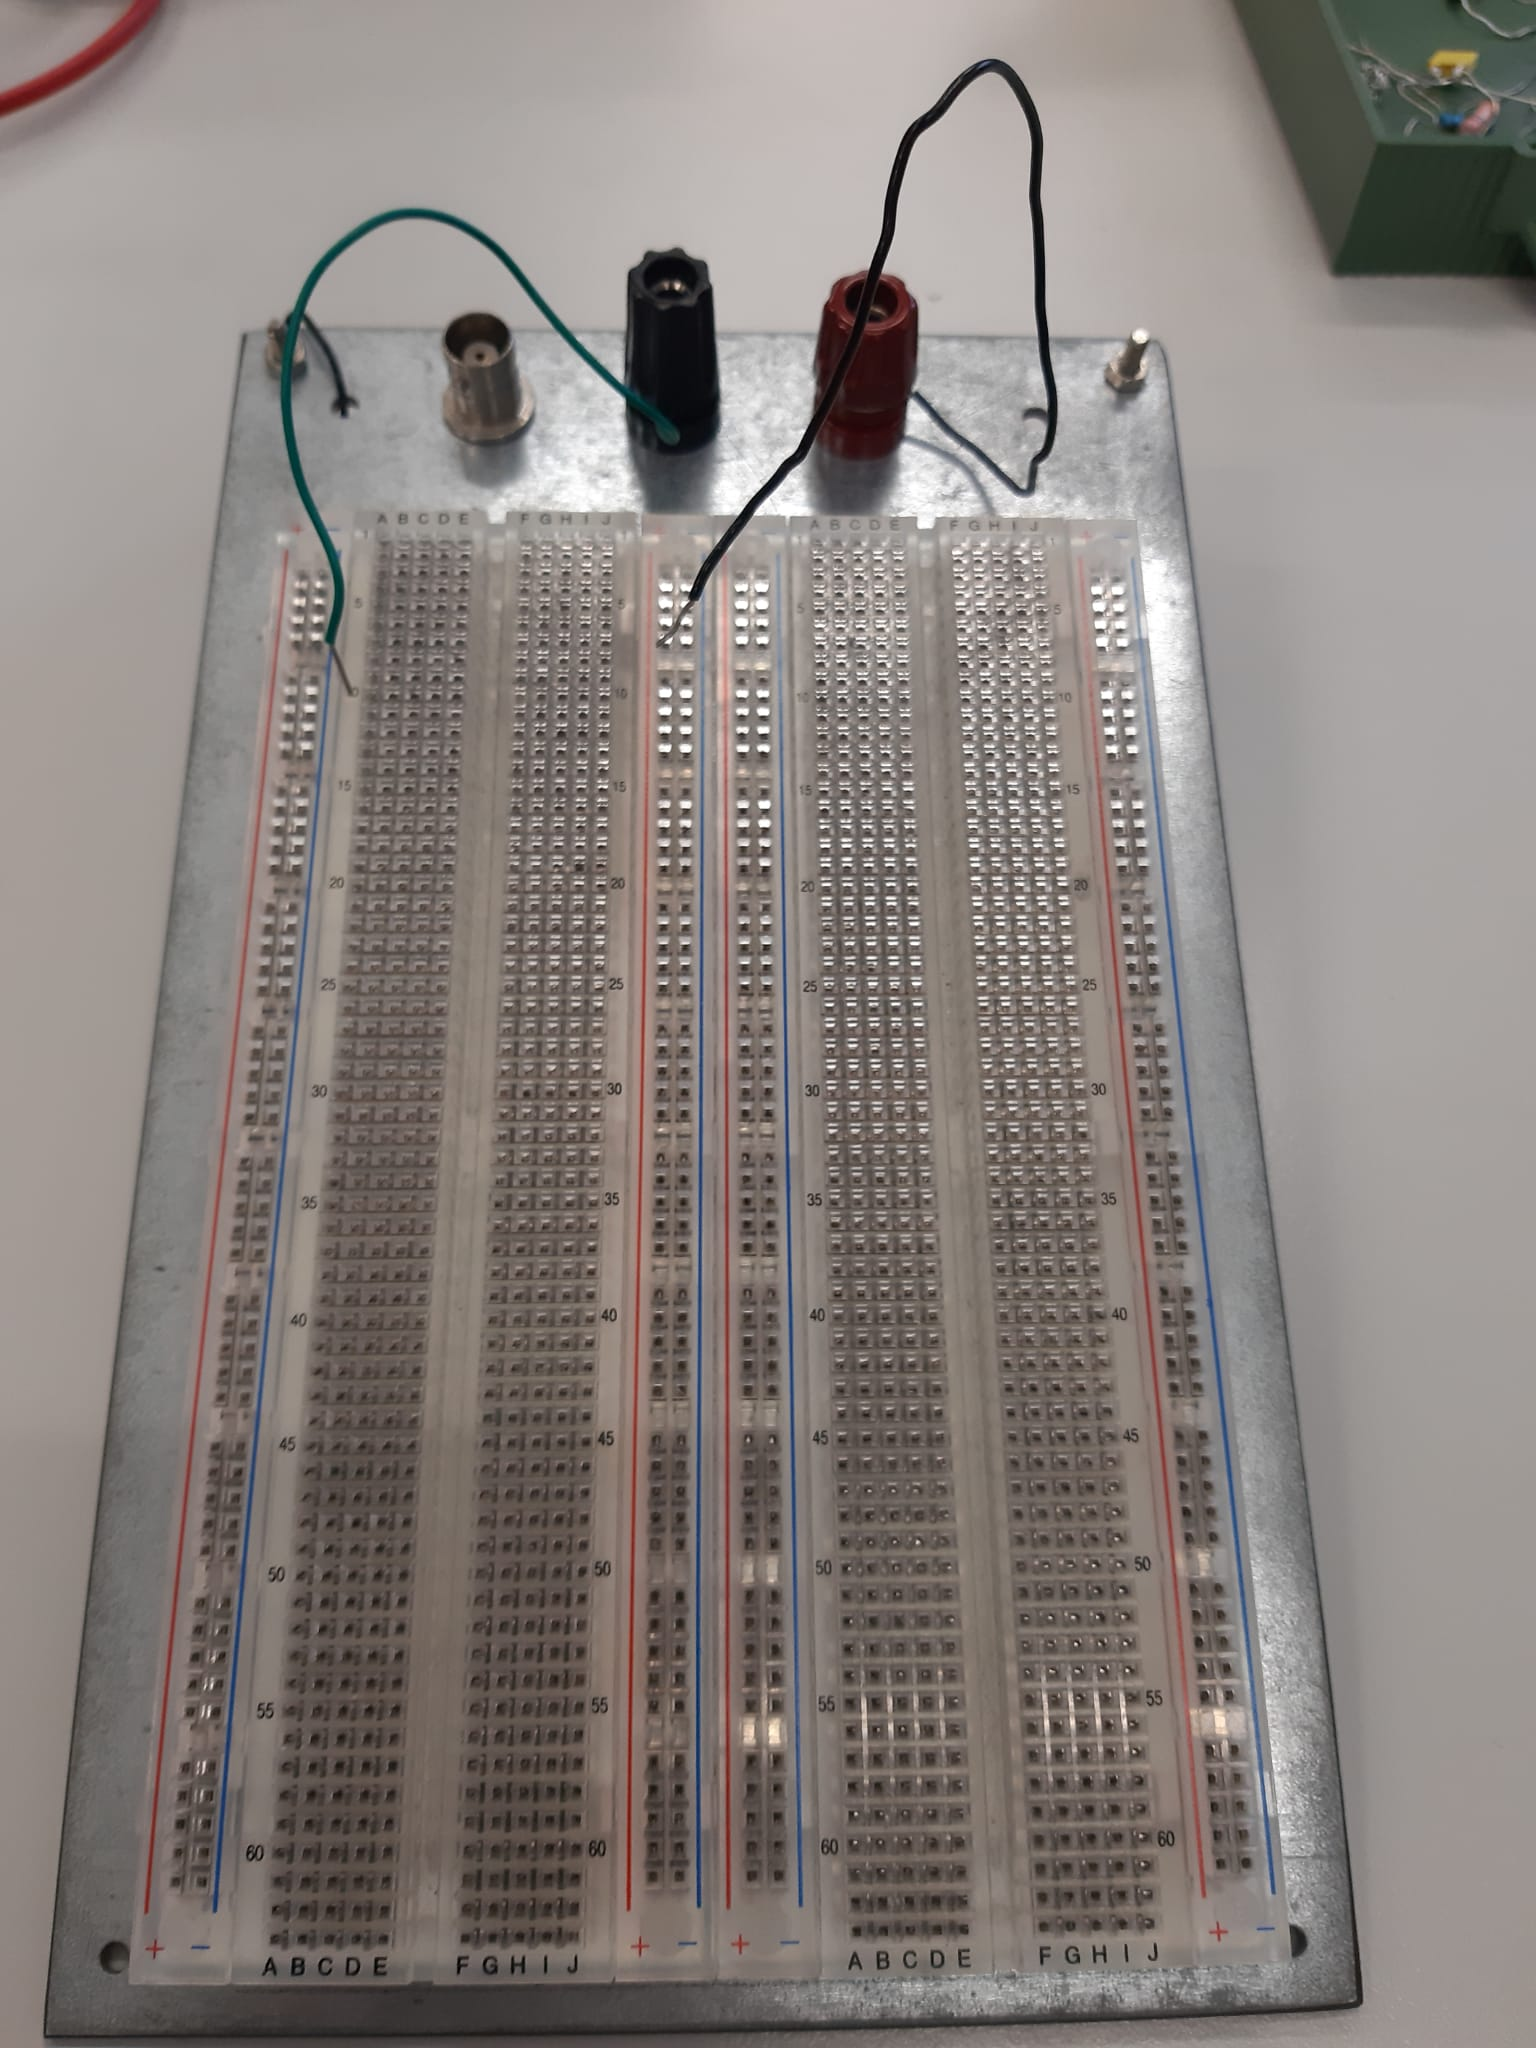
\includegraphics[scale=0.1]{Immagini/Circuitoooo.jpeg}
    \label{fig:my_label}
\end{figure}

La prima parte dell'esperienza si è concentrata sullo studio della strumentazione di laboratorio, studio finalizzato ad utilizzare configurazioni adeguate nelle parti successive. E' stato, infatti, necessario verificare che il multimetro usato come Voltmetro fosse ben progettato, cioè che avesse la caratteristica di possedere una resistenza in parallelo grande. Analogamente, è stato necessario verificare che il multimetro usato come Amperometro avesse la caratteristica di possedere una resistenza in serie piccola.
Successiavmente ci siamo concenrati sullo studio delle resistenze e della Legge di Ohm:

\begin{equation}
\frac{1}{R_{\parallel}}=\sum_{i=1}^{N}\frac{1}{R_{i}} \hspace{73 pt} R_{\perp}=\sum_{i=1}^{N}R_{i}
\end{equation}

\begin{equation}
V=R_{tot}I
\end{equation}

Infine, abbiamo studiato la Legge di Shockley, che descrive l'andamento di corrente per i diodi:

\begin{equation}
I=I_{0}(e^{qv/gK_b T}-1)
\end{equation}

indicando con \textit{q} la carica degli elettroni, con $K_b$ la costante di Boltzmann, con \textit{g} la costante che dipende dal tipo di diodo e con T la temperatura del diodo in Kelvin, corrispondente a quella dell'ambiente. Il termine di proporzionalità $I_0$ è detto \textit{intensità di corrente di saturazione}, il valore che ci aspettiamo di ottenere è molto piccolo in quanto si tratta di una corrente generata dai portatori di carica interni al diodo in diffusione dalla regione neutra alla regione di carica spaziale\footnote{Si tratta di una regione isolante all'interno di un semiconduttore drogato.}.
\section{Messa a fuoco}
Prima di procedere con gli esperimenti è stato necessario mettere a fuoco il telescopio. Dopo averlo puntato dalla finestra del laboratorio verso un punto di riferimento abbastanza lontano, abbiamo calibrato l'oggetto in modo da avere simultaneamente nitidi la croce di puntamento e il punto di riferimento stesso.
Poichè non era possibile bloccare la componente del telescopio, determinati movimenti dello spettrometro hanno più volte modificato la messa a fuoco, rendendo necessaria la ricalibrazione dello strumento più volte durante l'esperienza.

\section{Studio attraverso il prisma}
In primo luogo abbiamo fatto incidere il fascio collimato, proveniente da una lampada a Hg, su una delle facce ottiche del prisma e abbiamo ruotato l'oggetto analizzatore fino ad osservare l'angolo di inversione.
Prima di procedere è stato però necessario misurare l'angolo al vertice del prisma, ovvero l'angolo tra le due facce ottiche, riportadone la base su un foglio e osservando la congruenza di tutti i lati a meno di un errore di un millimetro.
L'angolo al vertice è risultato, quindi, essere di $\alpha$\,=\,60°.
Preso come zero l'angolo di allineamento, ovvero l'angolo per cui le due lenti permettevano una visione nitida del raggio luminoso, abbiamo proceduto misurando l'angolo di minima deviazione per ogni linea distinguibile:

\begin{table}[h!]
    \centering
    \begin{tabular}{cc}
    \toprule
    $\vartheta$ & angolo totale $\delta$ (rad)\\
    \midrule
    90°	0' &0,854\\
    90°	20' &0,860\\
    90°	40' &0,866\\
    91°	20' &0,877\\
    91°	23' &0,878\\
    92°	24' &0,896\\
    93°	20' &0,912\\
    93°	35' &0,916\\
\bottomrule
    \end{tabular}
    \caption{}
    \label{tab:my_label}
\end{table}
\noindent
%io anzichè mettere il numero della linea metterei più il range di colore

Da questi valori abbiamo ricavato l'indice di rifrazione per ogni lunghezza d'onda attraverso la formula:

\begin{equation}
n=\dfrac{\sin\left(\dfrac{\delta+\alpha}{2}\right)}{\sin\left(\dfrac{\alpha}{2}\right)}
\label{eq 2}
\end{equation}
Dall'Eq. \ref{eq 2} si può stimare l’incertezza su $n$ propagando l'errore sull'angolo
$$
\sigma^2_n = \left|\dfrac{\partial n}{\partial\delta} \right|^2\sigma^2_{\delta}
$$
\begin{equation}
    \sigma_{n}^{2}=\frac{1}{4}\left(\frac{1}{\sin ^{2}\left(\frac{\alpha}{2}\right)}-n^{2}\right)\sigma_{\delta}^{2}
\end{equation}
La seguente tabella mostra i risultati ottenuti

\begin{table}[h!]
    \centering
    \begin{tabular}{ccc}
    \toprule
    \textit{n} & $\lambda (\angstrom)$& $\sigma_n$ ($10^{-5}$)\\
    \midrule
    1,6276	&4046,56 &  94\\
    1,6309	&4339,22 &  94\\
    1,6343	&4347,49 &  93\\
    1,6410	&4358,33 &  91\\
    1,6415	&5460,73 &  91\\
    1,6515	&5769,60 &  89\\
    1,6607	&5790,66 &  87\\
    1,6631	&7081,90 &  86\\
\bottomrule
    \end{tabular}
    \caption{Indici di rifrazione con relativo errore}
\end{table}
\noindent
Infine abbiamo realizzato un fit lineare dei parametri al fine di stimare i coefficienti della legge di Cauchy al secondo ordine. I risultati del fit sono riportati di seguito.
\begin{figure}[h!]
    \centering
    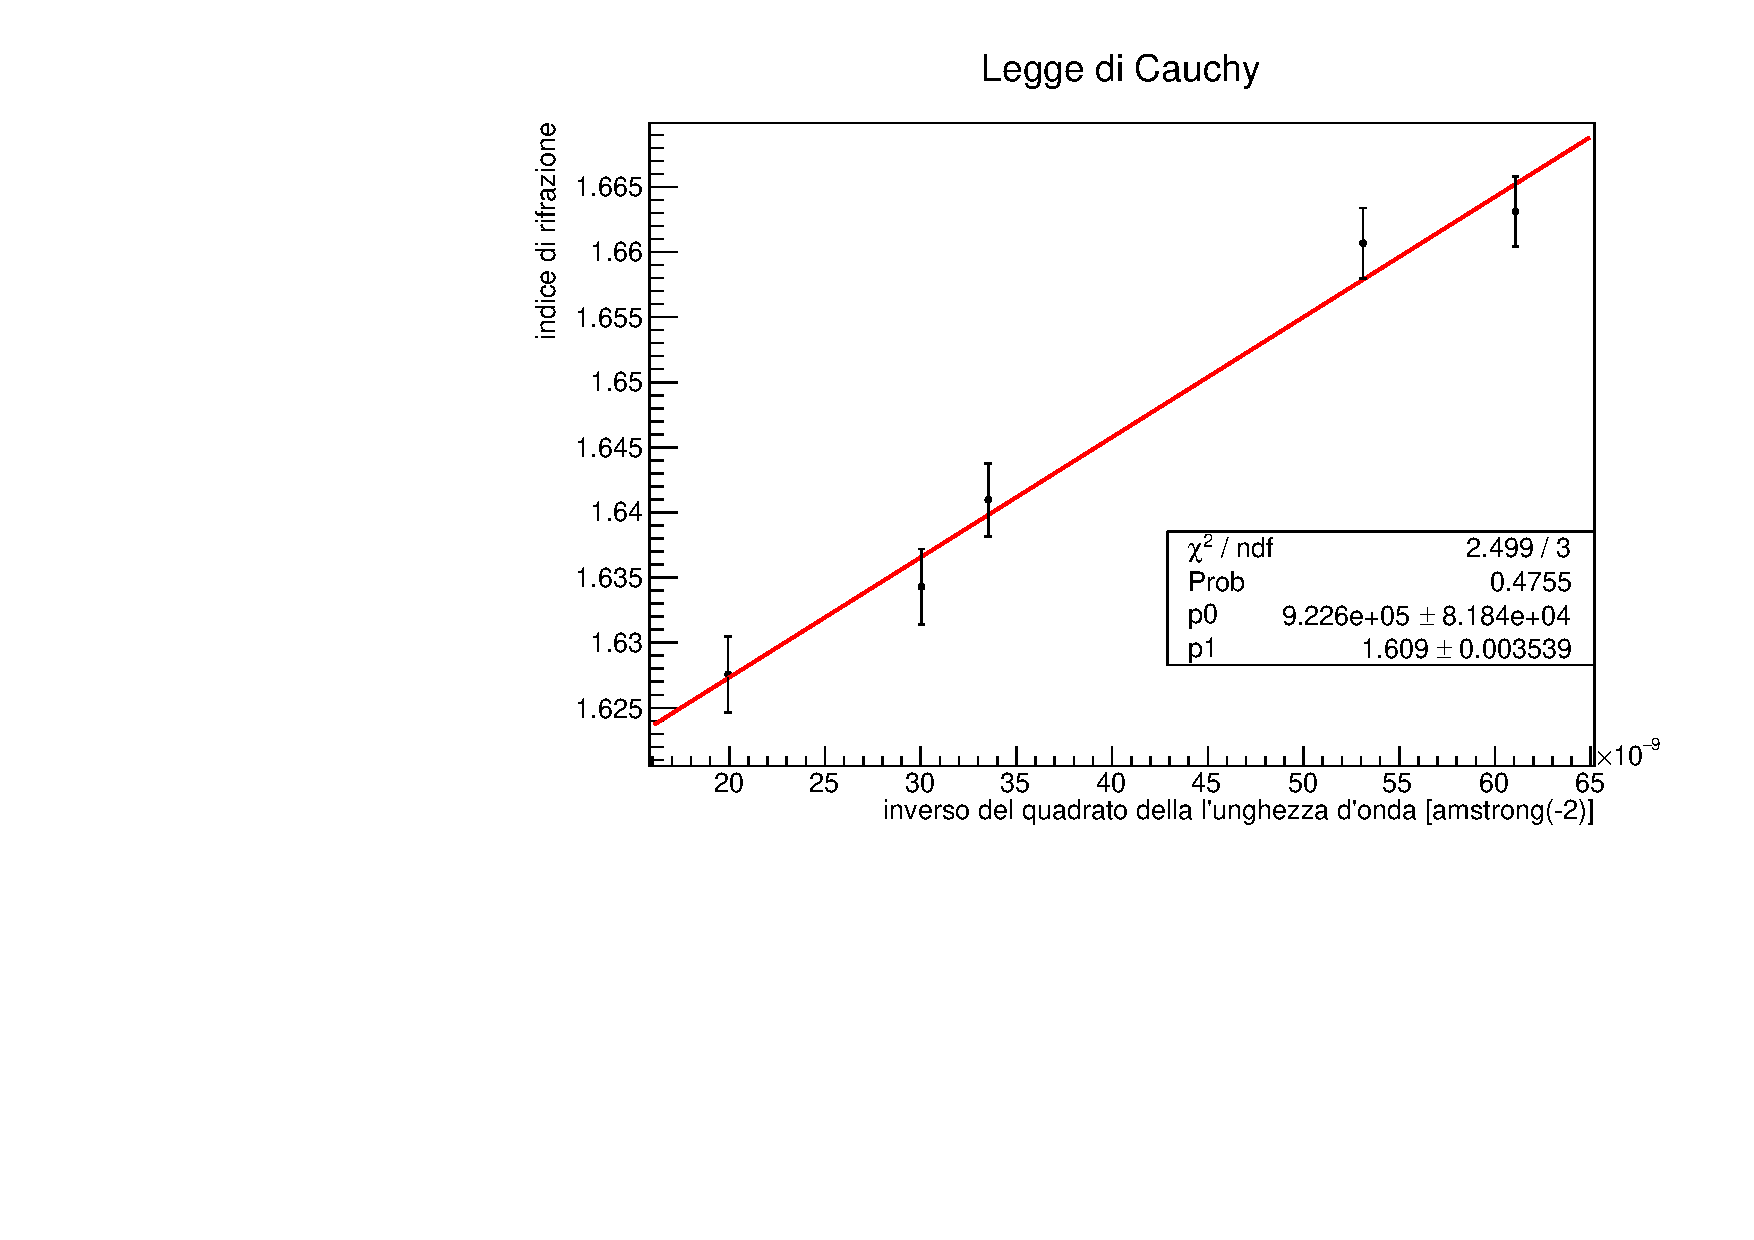
\includegraphics[scale=.4]{Immagini/Legge Cauchy.pdf}
    \caption{Il parametro A della legge di Cauchy qui è riportato come p1, mentre B come p0.}
\end{figure}

\noindent
Avendo una probabilità di $\chi^2$ maggiore di $0.05$, il fit viene considerato accettabile, la legge di Cauchy viene considerata verificata ed i parametri che la descrivono vengono stimati come:
$$
A = 1,609 \pm 0,003\qquad B= (92,26\pm 8,184)\times 10^{4}\,\angstrom^{-2}   \qquad \rho_{AB}= 1.2527\times 10^{-5}
$$
\section{Studio attraverso il reticolo}
Quando della luce incide perpendicolarmente su un reticolo di diffrazione, si viene a creare una figura di interferenza simmetrica rispetto alla direzione di incidenza. La posizione dei punti di interferenza costruttiva (detti massimi) segue la legge \ref{rifrazione}. La luce però non era perfettamente incidente, è dunque possibile considerare l'angolo $\alpha$ di incidenza e scrivere
$$
\sin(\vartheta -\alpha)=n\dfrac{\lambda}{d}
$$
Misurando gli angoli che compaiono in questa relazione, è possibile stimare il passo del reticolo oppure il suo reciproco, di cui in questo caso si conosce il valore con precisione assoluta.
\subsection{Raccolta e analisi dati}
Per svolgere l'esperienza sono stati utilizzati reticoli diversa densità di fenditure, precisamente $300$, $600$ e $1200$ fenditure per millimetro (questi valori corrispondono all'inverso del passo del reticolo).

Per ognuno di essi è stato necessario calibare lo spettrometro in modo che gli angoli dei massimi dello stesso ordine fossero alla stessa distanza angolare dal riferimento $\vartheta_0=\ang{63}\,35'$ nel limite di incertezze sperimentali. La seguente tabella riassume le misure di calibrazione
\begin{table}[h!]
    \centering
    \begin{tabular}{cc}
    \toprule
         Reticolo & $\vartheta_{max}$ (dx/sx)$-\vartheta_0$ \\
         \midrule
         300 & \ang{32}\,30'\\
             & -\ang{32}\,30'\\
        \midrule
         600 &  \ang{46}\,0'\\
          &-\ang{45}\,17'\\
        \midrule
        1200 & \ang{45}\,10'\\
        & -\ang{45}\,2'\\
    \bottomrule
    \end{tabular}
    \caption{}
    \label{tab:my_label}
\end{table}
Dopo questa operazione abbiao misurato gli angoli dei massimi di interferenza meglio individuabili. La seguente tabella mostra i dati raccolti in questa fase
\begin{table}[h!]
    \centering
    \begin{tabular}{cccc}
    \toprule
    Reticolo & $\ang{1}$ ordine & $\ang{2}$ ordine & $\ang{3}$ ordine \\
    \midrule
    300     & \ang{73}\,48’ & \ang{84}\,38'&\ang{96}\,5'\\
    \midrule
    600     &\ang{84}\,32' & \ang{109}\,35' & \\
    \midrule
    1200 & \ang{108}\,35' & &\\
    \bottomrule
    \end{tabular}
    \caption{}
    \label{tab:my_label}
\end{table}
\subsection{Correzione sull'angolo}
La non perpendicolarità della luce incidente può essere corretta introducento l'angolo $\alpha$ il cui valore viene ricavato da considerazioni ottico geometriche da cui si giunge alla seguente relazione
\begin{equation}
    \tan\alpha=\dfrac{\sin\theta_{+}+\sin\theta_{-}}{2-\cos\theta_{+}-\cos\theta_{-}}
\end{equation}
dove $\theta_\pm$ sono gli angoli, a destra e a sinistra, a cui si trovano i massimi della figura di interferenza. Da questa relazione può essere ricavata l'incertezza relativa a questa grandezza che si trova essere
\begin{equation}
\sigma_{\alpha}^{2}=\frac{\left(2 \cos \theta_{+}-\cos \left(\theta_{+}-\theta_{-}\right)-1\right)^{2}+\left(2 \cos \theta_{-}-\cos \left(\theta_{+}-\theta_{-}\right)-1\right)^{2}}{\left(1+\tan ^{2} \alpha\right)^{2}\left(2-\cos \theta_{+}-\cos \theta_{-}\right)^{4}} \sigma_{\theta}^{2}
\end{equation}
La seguente tabella riassume i risultati raccolti
\begin{table}[h!]
    \centering
    \begin{tabular}{ccc}
    \toprule
    Reticolo & $\alpha$ & $\sigma_\alpha$\\
    \midrule
    300     &0' &5' \\
    \midrule
    600     &50' &2'\\
    \midrule
    1200 & 7' & 2' \\
    \bottomrule
    
    \end{tabular}
    \caption{}
    \label{tab:my_label}
\end{table}
\subsection{Verifica della legge di diffrazione \label{paragrafo 3}}
\begin{figure}[h!]
    \centering
    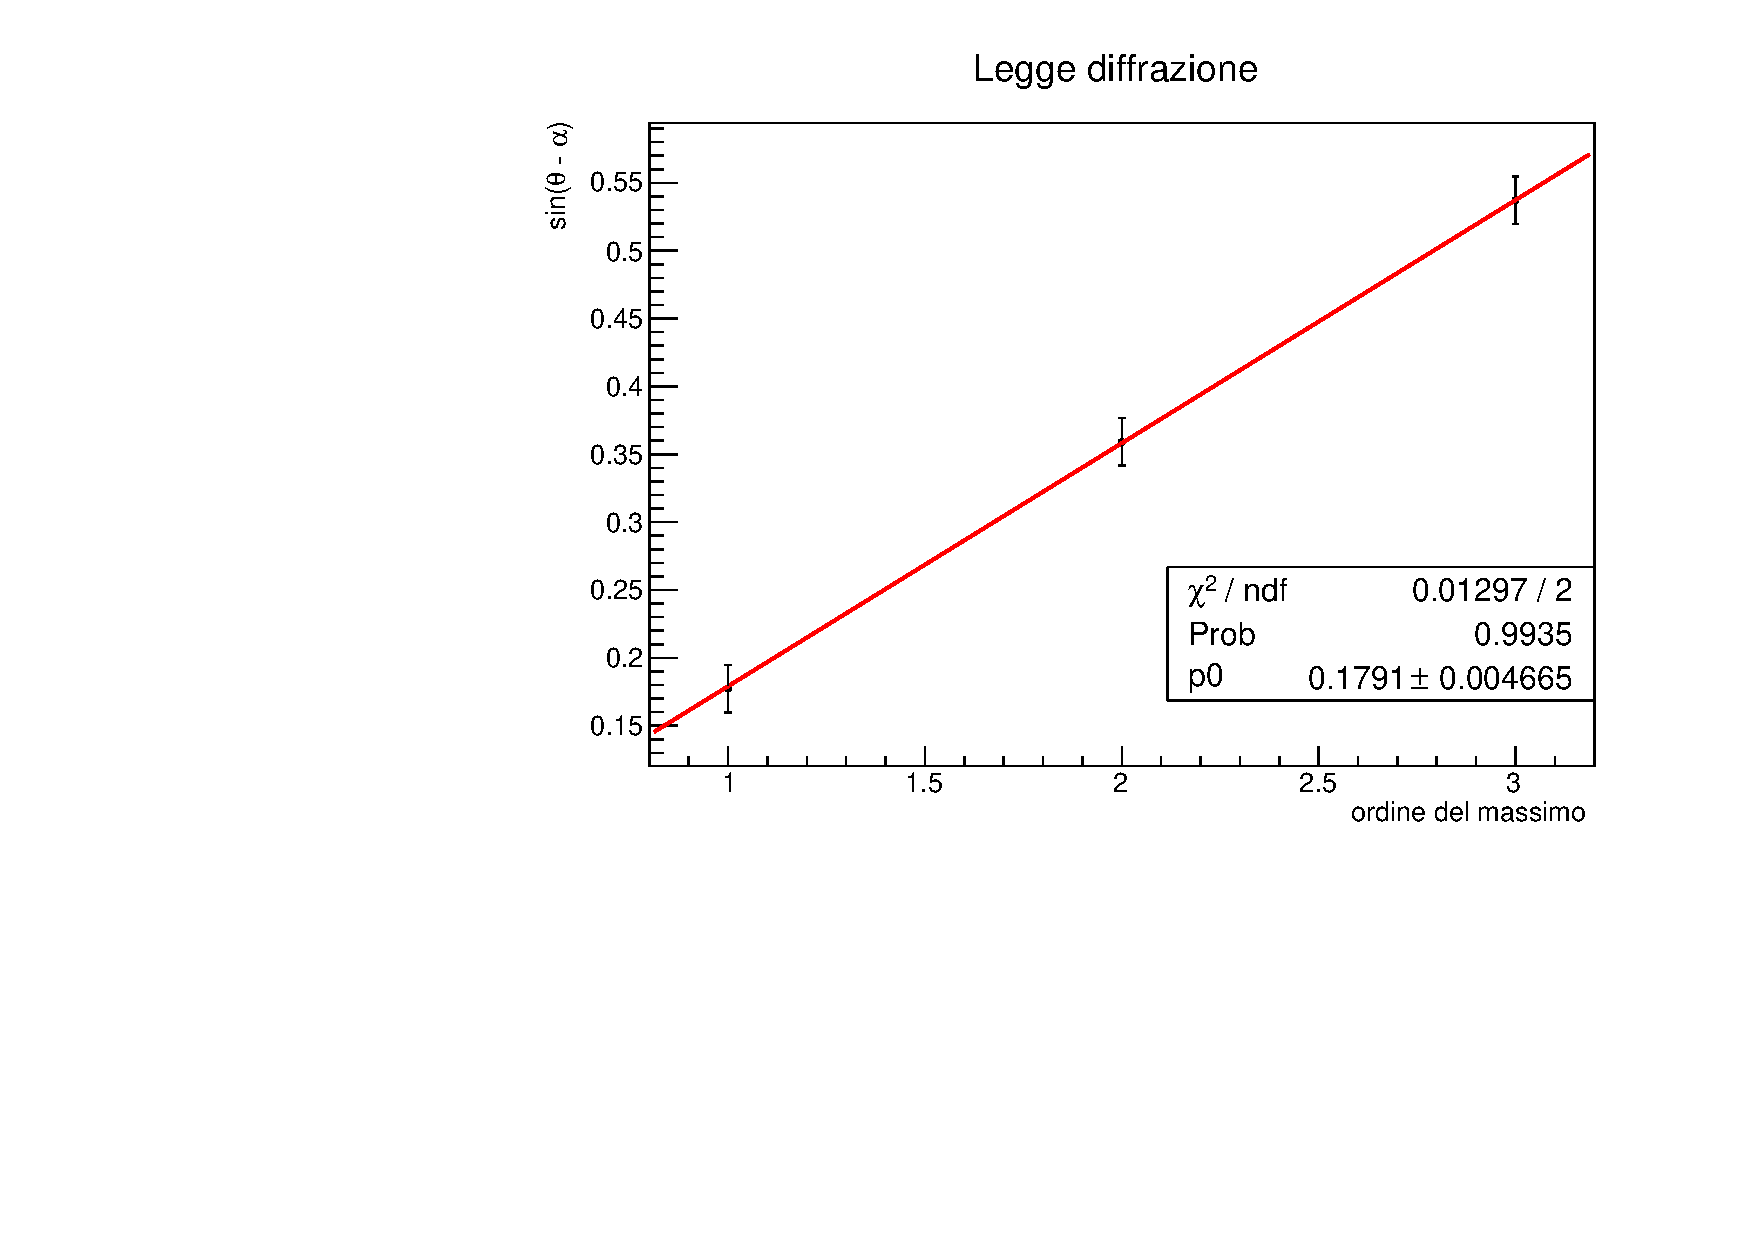
\includegraphics[scale=.6]{Immagini/legge diffrazione.pdf}
    \caption{}
    \label{fit rifrazione}
\end{figure}

Siccome utilizzando il reticolo da $300\,\frac{\text{fend.}}{\text{mm}}$ è possibile ricavare massimi di tre ordini differenti, la stima del suo passo può essere effettuata interpolando l'equazione
$$
\sin(\vartheta-\alpha)=n\dfrac{\lambda}{d}
$$
In questo modo si verifica anche la legge stessa. Chiamato $\beta=\vartheta-\alpha$ l'angolo effettivo del massimo rispetto alla normale del reticolo, si può dire che 
$$
\sigma^2_\beta = \sigma_\alpha^2+\sigma_\vartheta^2
$$
per poi effettuare il fit riportato nella Fig. \ref{fit rifrazione}. Da tale interpolazione si stima il valore caratteristico del reticolo dividendo per $\lambda$
$$
\dfrac{1}{d}=303,8\pm 0,5 \frac{\text{fend.}}{\text{mm}}
$$
Il valore ricavato di $1/d$ non è compatibile con il valore atteso di $300\,\frac{\text{fend.}}{\text{mm}}$ in quanto eseguendo il $t-$test di Student si trova che 
$$
t_s=\dfrac{\hat{\vartheta}-\vartheta_t}{\sigma_\vartheta}=7,6
$$

Questo fa presumere che la legge di diffrazione sia esatta (i dati sperimentali seguono effettivamente una proporzionalità lineare), ma che ci sia un errore nella stima del valore cercato. L’ipotesi più attendibile riguarda un errore nella stima di $\alpha$: dato che una sua variazione di pochi primi comporta un’importante variazione dei risultati, e dato che il supporto del reticolo non era vincolato in modo rigido ma libero di muoversi, si può supporre che nell’atto di misurazione degli angoli tale reticolo si sia leggermente spostato.
\subsubsection{Altri reticoli}
Siccome per gli altri reticoli non disponevamo di sufficienti misure per effettuare un'interpolazione affidabile abbiamo proceduto sitmando i parametri in maniera diretta
$$
\frac{1}{d}=\frac{1}{n \lambda} \sin (\theta-\alpha)
$$
$$
\sigma_{\frac{1}{d}}=\frac{1}{n \lambda} \cos (\theta-\alpha) \sqrt{\sigma_{\theta}^{2}+\sigma_{\alpha}^{2}}
$$
I risultati sono raccolti nella seguente tabella
\begin{table}[h!]
    \centering
    \begin{tabular}{ccc}
    \toprule
    Reticolo $(\frac{\text{fend.}}{\text{mm}})$ & $1/d$ $(\frac{\text{fend.}}{\text{mm}})$ & $\sigma_{\frac{1}{d}}$ $(\frac{\text{fend.}}{\text{mm}})$\\
    \midrule
         600 & 599,2 & 0,4 \\
         1200 &  1200,3 & 0,8\\
    \bottomrule
    \end{tabular}
    \caption{}
    \label{tab:my_label}
\end{table}
\\

In questo caso i valori sono accettabilmente compatibili con quelli attesi e ci permette di confermare la validità della legge di diffrazione, a discapito dell’errata stima fatta in precedenza.
\section{Studio gas ignoto}
Sostituendo la sorgente nota con una incognita, ci è stato possibile sfruttare la legge di Cauchy appena verificata per risalire al valore delle lunghezze d’onda che abbiamo osservato.
La procedura sperimentale è identica e consiste nella stima degli indici di rifrazione associati alle righe di emissione più intense della sorgente incognita.
\subsection{Prima sorgente ignota}
La seguente tabella riassume le misure raccolte
\begin{table}[h!]
    \centering
    \begin{tabular}{ccc}
    \toprule
    $n$ && $\lambda\,(\angstrom)$ $(10^{-5})$ \\
    \midrule
    1,66423  &&  95\\
    1,64990  &&  96\\
    1,64197  &&  98\\
    1,63546  &&  99\\
    1,63463  &&  996\\
    1,63295  &&  100\\
    1,63211  &&  100\\
    1,62992  &&  101\\
    1,62992  &&  101\\
    \bottomrule
    \end{tabular}
    \caption{}
    \label{tab:my_label}
\end{table}

A questo punto invertendo la legge di Cauchy è possibile risalire a $\lambda$ e la sua incertezza
\begin{equation}
\lambda= \sqrt{\dfrac{B}{n-A}}
\label{lambda}
\end{equation}
\begin{equation}
\sigma_\lambda^2=\frac{1}{4(n-A)^{2}}\left(\lambda^{2}\left(\sigma_{A}^{2}+\sigma_{n}^{2}\right)+2 \sigma_{A B}^{2}+\frac{\sigma_{B}^{2}}{\lambda^{2}}\right)
\label{sigma lambda}
\end{equation}
I risultati del fit sono riportati nella Figura \ref{confronto 1}.
\begin{figure}[h!]
    \centering
    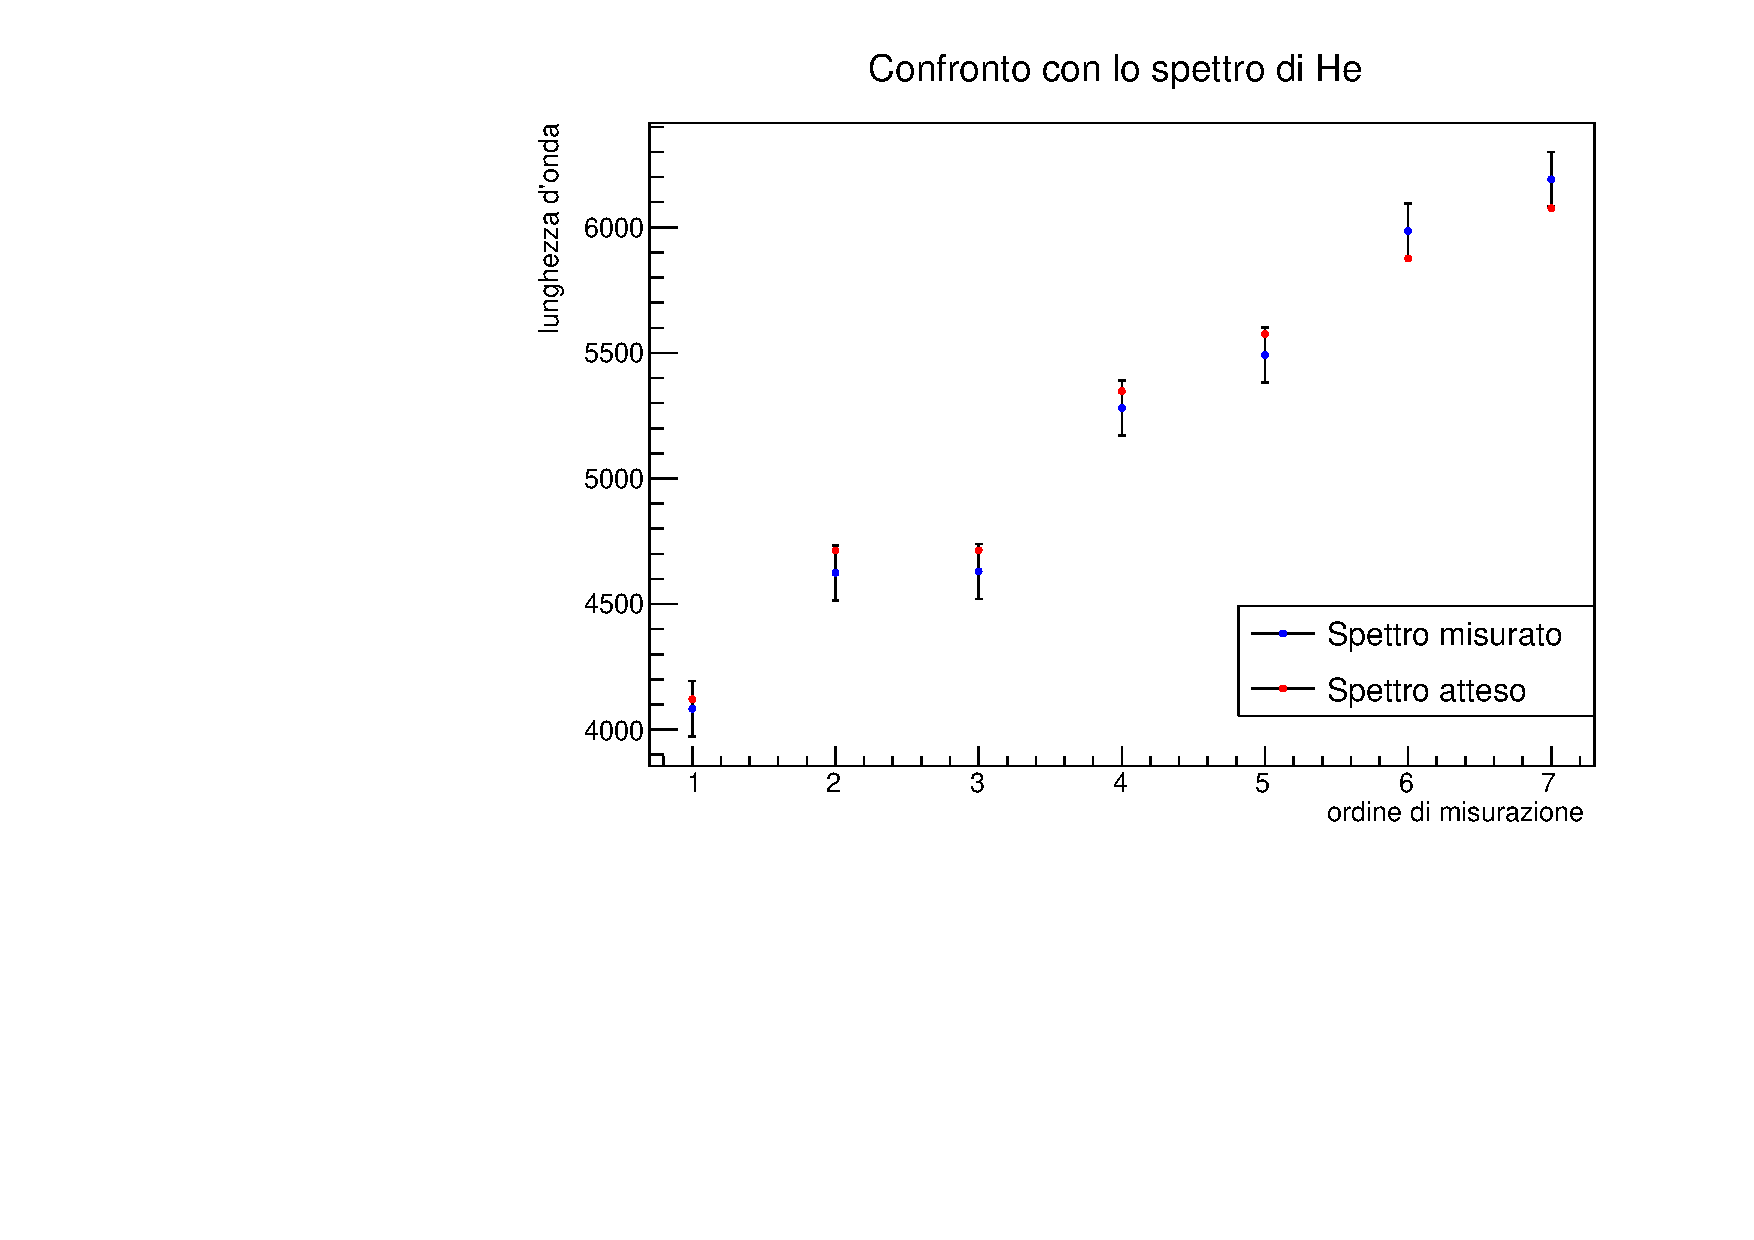
\includegraphics[scale=.4]{Immagini/Confronto 1.pdf}
    \caption{}
    \label{confronto 1}
\end{figure}
\subsection{Seconda sorgente ignota}
La tabella \ref{tabella 8} riassume le misure raccolte. Successivamente tramite le Eq. \ref{lambda} e \ref{sigma lambda} si ricavano i valori di $\lambda$ e $\sigma^2_\lambda$. I risultati del confronto sono riportati nella Figura  \ref{confronto 2}.
\begin{table}[h!]
    \centering
    \begin{tabular}{cc}
    \toprule
    $n$ & $\lambda$ ($\angstrom$)\\
    \midrule
    1,6350	&5946,74\\
    1,6370	&5730,32\\
    1,6450	&5056,89\\
    1,6587	&4301,91\\
    1,6613	&4194,11\\
    1,6662	&4012,93\\
    1,6734	&3782,16\\
    \bottomrule
    \end{tabular}
    \caption{}
    \label{tabella 8}
\end{table}
\begin{figure}[h!]
    \centering
    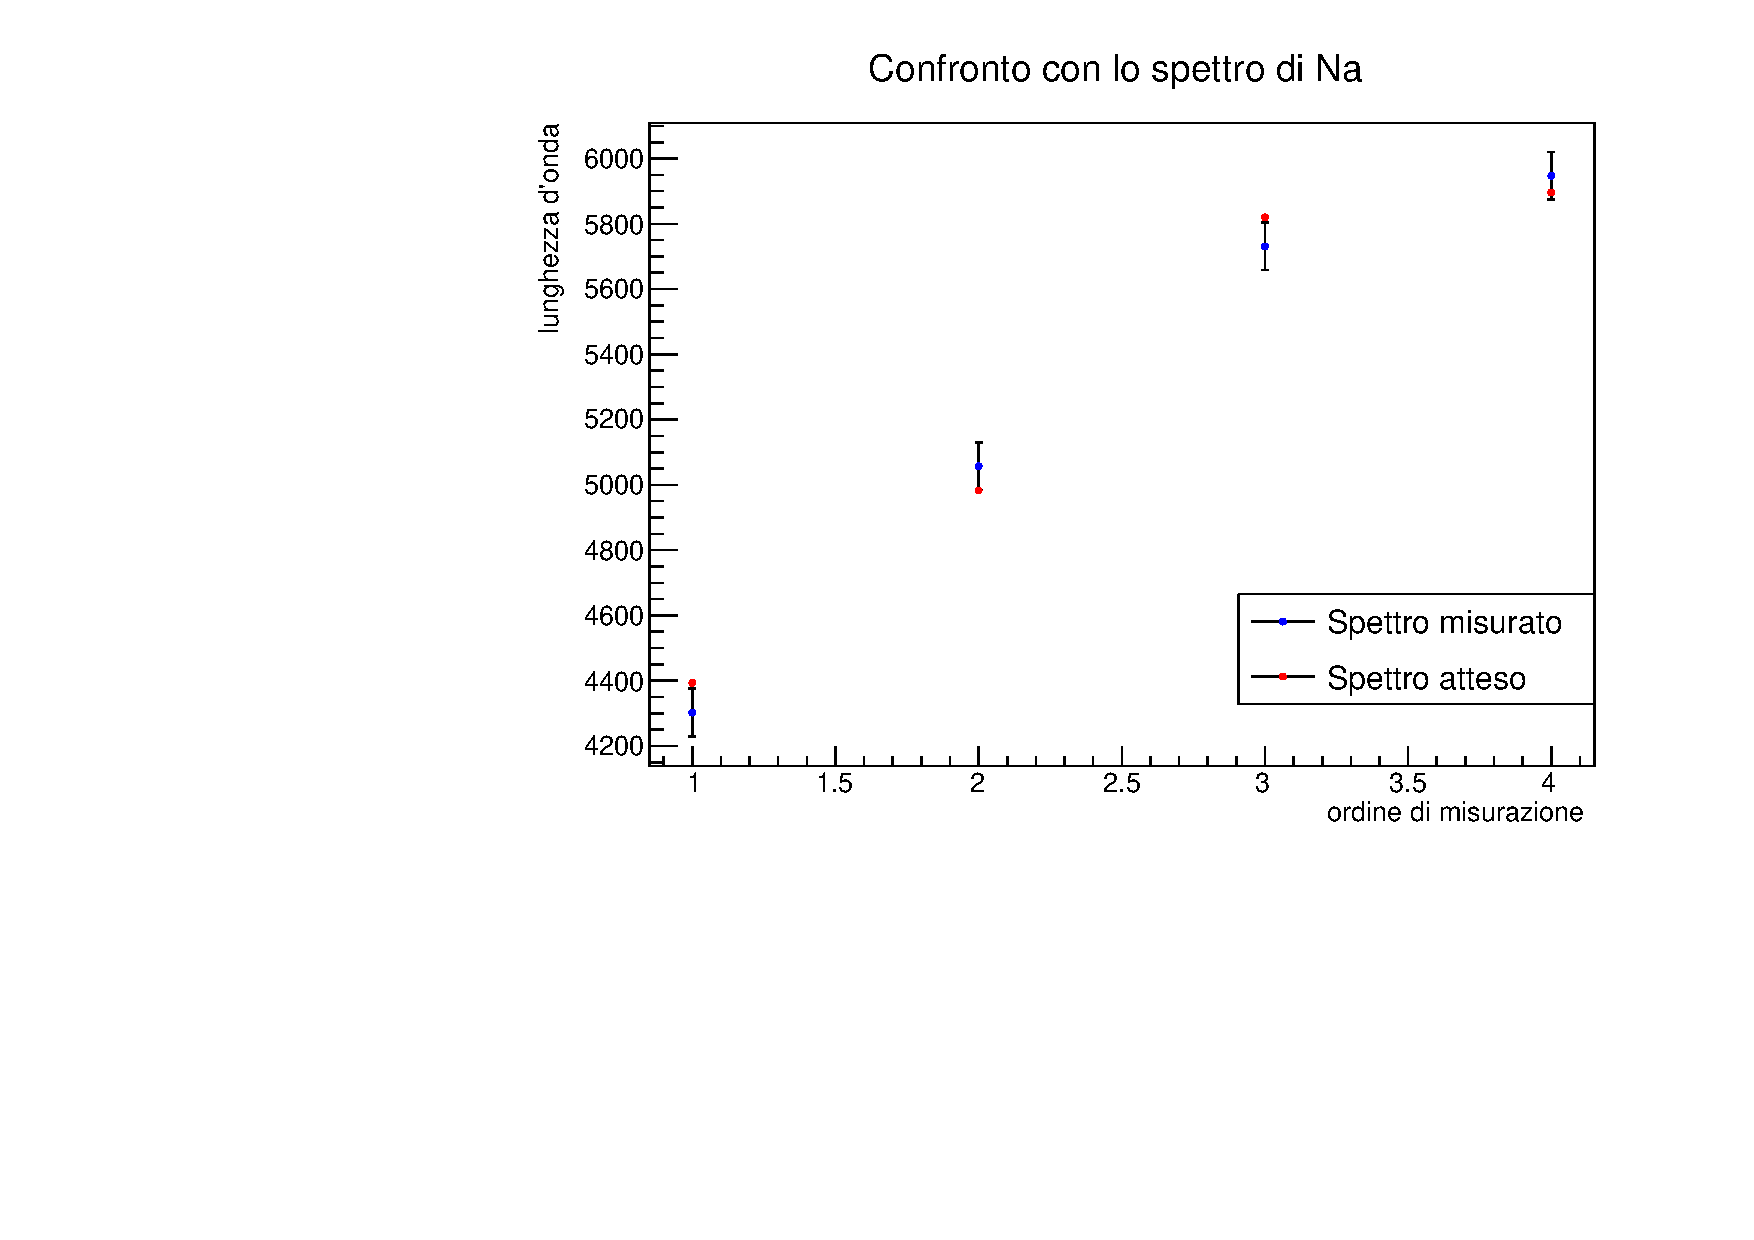
\includegraphics[scale=.4]{Immagini/Confronto 2.pdf}
    \caption{}
    \label{confronto 2}
\end{figure}
\subsection{Considerazioni sui gas determinati}
Confrontando i valori ottenuti con quelli tabulati per i gas nobili, si osserva una forte compatibilità con le righe di emissione dell’Elio e del Sodio, seppur con un certo bias. Si nota infatti che non è presente una regolarità nell'andamento della posizione della $\lambda$ misurata, se sopra se sotto, rispetto a ciò che ci si attende. Il seguente grafico mostra qualitativamente tale bias.

La natura di questo bias non è pienamente chiara: potrebbe trattarsi di una stima errata di $\vartheta_0$ o di $\alpha$, presente, quindi, fin dall’inizio dell’esperienza. Dato che abbiamo cercato di effettuare le misure nel modo più preciso possibile, un’ipotesi che è possibile avanzare riguarda la struttura geometrica del prisma: infatti, la presenza di vertici smussati potrebbe aver fatto sì che la luce non incidesse su uno spigolo perfettamente verticale ma su una superficie lievemente irregolare.
Questa ipotesi può trovare conferma nella forma righe di emissione che, viste dal telescopio, sono risultate essere incurvate e non perfettamente verticali. Ciò nonostante, dare una stima quantitativa di questa perturbazione risulta essere difficoltoso e quindi la misura viene giudicata allo stesso modo accettabile.

\section{Conclusioni}
Lo scopo di questa esperienza è stato quello di studiare e verficare relazioni e leggi riguardanti resistenze e diodi. In primo luogo è stata condotta una verifica sulle due configurazioni, quella con il voltmetro e quella con l'amperometro, al fine di analizzare i loro comportamenti rispetto alle configurazioni ideali. Per l'amperometro i risultati ottenuti risultano congruenti con quelli aspettati, cosa che invece non accade con il voltmetro. Crediamo che la causa di ciò possa essere dovuta a due principali fattori. In primis riteniamo possibile che la resistenza scelta, la quale era necessario fosse confrontabile con quella del voltmetro, potrebbe non essere stata tale e che, quindi, l'errore sull'ordine di grandezza potrebbe essere stato causato da quello. Come seconda fonte di errore riconduciamo il fatto che, per identificare le resistenze, ci siamo serviti del tool online menzionato nell'introduzione, i cui valori potrebbero non corrispondere a quelli reali, inserendo quindi un possibile errore sistematico nei nostri risultati. A causa di tale incongruenza, in esperienze che fornivano la possibilità di scegliere la configurazione, abbiamo sempre preferito utilizzare quella con l'amperometro. Lo studio sulla relazione evidenziata da Ohm risulta corretta, nonostante il $\chi^2$ risulti molto bassa. La causa più probabile di questo fenomeno potrebbe essere ricercata in una sottostima degli errori, dovuta al nostro modo di identificare i valori delle resistenze. Nonostante questa possibile fonte di errore, lo studio sul partitore resistivo ha portato risultati congruenti rispetto al nostro studio teorico riguardo alle relazioni sulle resistenze. Infine, anche l'analisi sul diodo risulta congruente rispetto alla relazione ipotizzata, con un $\chi^2$ ridotto di circa 0.82. Riteniamo che l'esperimento potrebbe essere riprodotto con risultati più soddisfacenti se si procedesse a misurare le resistenze in maniera differente. 

\end{document}